\subsection{Non-economic Applications}\label{subsec:nonecon}\hypertarget{nonecon}{}

This section highlights elements of epidemiological modeling in other fields that might be of most value to economists.   \ifInBook{}{(See the literature map in Figure \ref{fig:graph_other}).}  We focus on three areas:
\begin{verbatimwrite}{./Slides/NonEcon}
  \begin{enumerate}
  \item the spread of news, fake news, and rumors
  \item the diffusion of scientific ideas
  \item the dissemination pattern of internet content such as memes
  \end{enumerate}
\end{verbatimwrite}
  \begin{enumerate}
  \item the spread of news, fake news, and rumors
  \item the diffusion of scientific ideas
  \item the dissemination pattern of internet content such as memes
  \end{enumerate}


\ifInBook{}{
  \begin{figure}[!ht]
    \centering  % [h!]
    \caption{ ~Other fields related to epidemiological models}
    \label{fig:graph_other}
    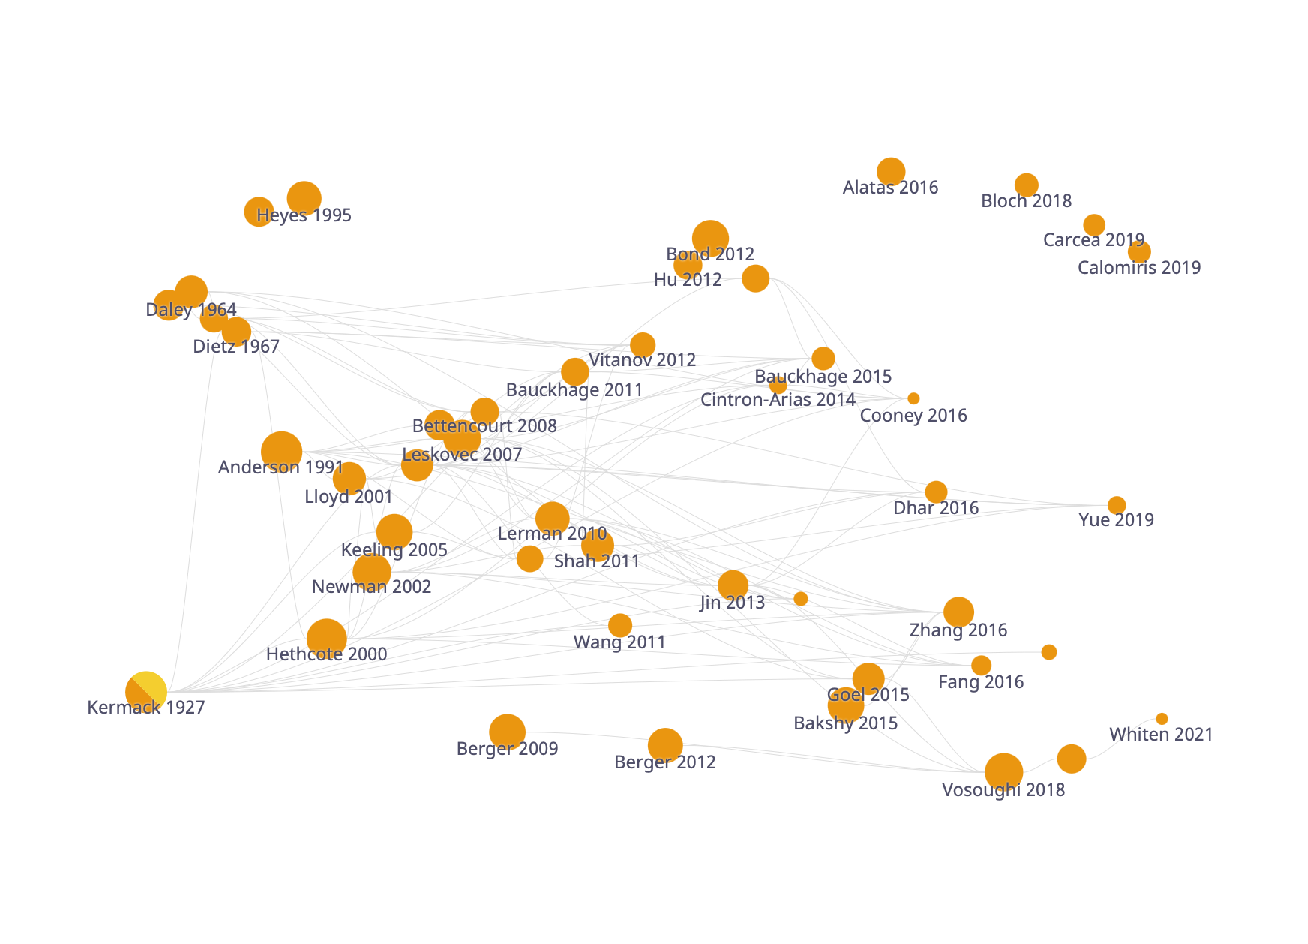
\includegraphics[width=\textwidth]{./figures/graph_other}
    \begin{flushleft}{\footnotesize Note: This graph includes selective non-economic research surveyed in this chapter, including epidemiological models of rumor/news/online content/scientific ideas. See \href{https://app.litmaps.co/shared/07C0B3F0-B4A9-4627-923C-857F1ABFD2D3}{here} for its interactive version.}
    \end{flushleft}
  \end{figure}
}

\cite{daley1964epidemics}'s proposal that rumors spread like diseases spurred a literature exploring variants of the classical epidemiological model.  A highly cited example (\cite{jin2013epidemiological}) \ifInBook{}{augments the usual three compartments of Susceptible, Infected, and Exposed with another compartment of skeptics, and}
estimates a model using the diffusion patterns of news about eight real events among Twitter users, including the Boston marathon bombings  and the resignation of Pope Benedict, and rumors such as the Mayan doomsday.  In each case, the model matches the dynamics reasonably well. \ifInBook{}{(See Figure \ref{fig:news_curve}).}

% \begin{center}[Insert Figure \ref{fig
% \begin{center}[Insert Figure \ref{fig:news_curve}  here]\end{center}
\begin{verbatimwrite}{./Slides/FigureNewsCurve}
  \begin{figure}[!ht] \centering  % [h!]
    \caption{ ~Spreading of news and rumors: Jin et al (2013)}\nocite{jin2013epidemiological}
    \label{fig:news_curve}
    \centerline{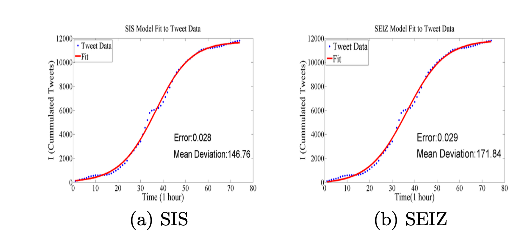
\includegraphics[width=\textwidth]{./figures/Doomsday}}
    \begin{flushleft}{\footnotesize Note: This graph is reproduced from \cite{jin2013epidemiological}, showing their fitted SIS and SEIZ model of the counts of Twitter posts related to the ``Mayan Doomsday'' rumor, which was widely circulated before December 21, 2012.}
    \end{flushleft}
  \end{figure}
\end{verbatimwrite}%%%Slides

\ifInBook{}{
  \begin{figure}[!ht] \centering  % [h!]
    \caption{ ~Spreading of news and rumors: Jin et al (2013)}\nocite{jin2013epidemiological}
    \label{fig:news_curve}
    \centerline{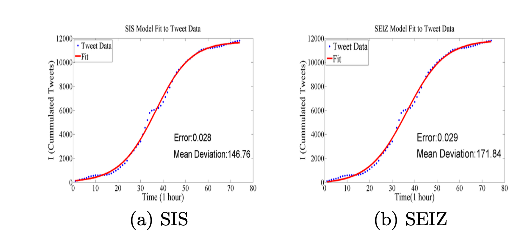
\includegraphics[width=\textwidth]{./figures/Doomsday}}
    \begin{flushleft}{\footnotesize Note: This graph is reproduced from \cite{jin2013epidemiological}, showing their fitted SIS and SEIZ model of the counts of Twitter posts related to the ``Mayan Doomsday'' rumor, which was widely circulated before December 21, 2012.}
    \end{flushleft}
  \end{figure}

}
\IfPrivate{\href{https://www.science.org/doi/10.1126/science.aap9559}{\cite{vosoughi2018spread}}}{\cite{vosoughi2018spread}} found that falsehood spreads on the internet faster than the truth, possibly because the interesting falsehoods have a greater capacity to produce emotional arousal.  Similarly, \IfPrivate{\href{https://journals.sagepub.com/doi/10.1509/jmr.10.0353}{\cite{berger2012makes}}}{\cite{berger2012makes}} claim that ``content that evokes high-arousal positive (awe) or negative (anger or anxiety) emotions is more viral. Content that evokes low-arousal, or deactivating, emotions (e.g., sadness) is less viral.'' \IfPrivate{\href{https://arxiv.org/abs/1805.12512}{\cite{zannettou2018origins}}}{\cite{zannettou2018origins}} found that the content of a meme affects its virality: racist and political memes are particularly viral.

\cite{kohlhasasymmetric} attempt to explain evidence that people seem to underreact to events that are not very surprising, but overreact to surprising events.  The authors attempt to model this using a combination of ideas from Sims's rational inattention framework and the Bordalo-Shleifer diagnostic expectations model, but to the extent that surprising events elicit emotional arousal, this paper may also be connected to the noneconomic literature.  %Whether or not this speculative link is correct, a broader point is that a unifying way to talk about these ideas is to characterize them all as being about ways of quantifying the degree of ``infectiousness'' of various kinds of content.

% About 126,000 rumors were spread by ∼3 million people. False news reached more people than the truth; the top 1% of false news cascades diffused to between 1000 and 100,000 people, whereas the truth rarely diffused to more than 1000 people. ...We found that false news was more novel than true news, which suggests that people were more likely to share novel information. Whereas false stories inspired fear, disgust, and surprise in replies, true stories inspired anticipation, sadness, joy, and trust. Contrary to conventional wisdom, robots accelerated the spread of true and false news at the same rate, implying that false news spreads more than the truth because humans, not robots, are more likely to spread it.

\IfPrivate{\href{https://github.com/iworld1991/EpiExp/blob/master/Literature/allcott2017social.pdf}{\cite{allcott2017social}}}{\cite{allcott2017social}} used a post-2016-election U.S.\ survey to analyze the importance of social media for fake news consumption, exposure to fake news, and partisan composition.  The paper models profit-maximizing firms who supply fake news in order to appeal to consumers subject to confirmation bias. This seems a natural extension of standard epidemiological models to incorporate the production side of the content -- ``infectiousness'' of certain ideas in subpopulations is an incentive for the production of content that will become ``viral'' because of a high reproductive number in the targeted subpopulation.

Another potential determinant of the degree to which ideas spread is explored in \IfPrivate{\href{https://www.kdd.org/exploration_files/8._CR.10.Misinformation_in_social_media_-_Final.pdf}{\cite{acemoglu2010spread}}}{\cite{acemoglu2010spread}}, who show show that the presence of ``forceful'' agents (who are immune to others' opinions) may lead to the persistence of misinformation. The key insight is that heterogeneity in infectiousness can reflect characteristics of the sender (`forcefulness') as well as the receiver.

Epidemiological models have also been effectively used to study the spread of scientific ideas.    For example,  \IfPrivate{\href{https://github.com/iworld1991/EpiExp/blob/master/Literature/bettencourt2006power.pdf}{\cite{bettencourt2006power}}}{\cite{bettencourt2006power}} find that epidemiological models perform well in explaining the the spread of Feynman diagrams through theoretical physics communities\ifInBook{.}{.}% (see Figure \ref{fig:science_ideas_curve})
 \ifInBook{}{That paper uses an SEIR model where E represents the exposed state, and a SEIZ model where Z represents skeptics (mutually exclusive with being infected) who held competing ideas. Introducing skeptics generates an additional steady state of the model where competing ideas coexist. This differs from two-compartment and three-compartment models, in which typically the system converges to a single state.}

\begin{verbatimwrite}{./Slides/FigureScienceIdeasCurve}
  \begin{figure}[!ht] \centering
    \caption{ ~Diffusion of scientific ideas: \href{http://web.mit.edu/dikaiser/www/BAKC.PhysA.pdf}{Bettencourt et al (2006)}}\nocite{bettencourt2006power}
    \label{fig:science_ideas_curve}
    \centerline{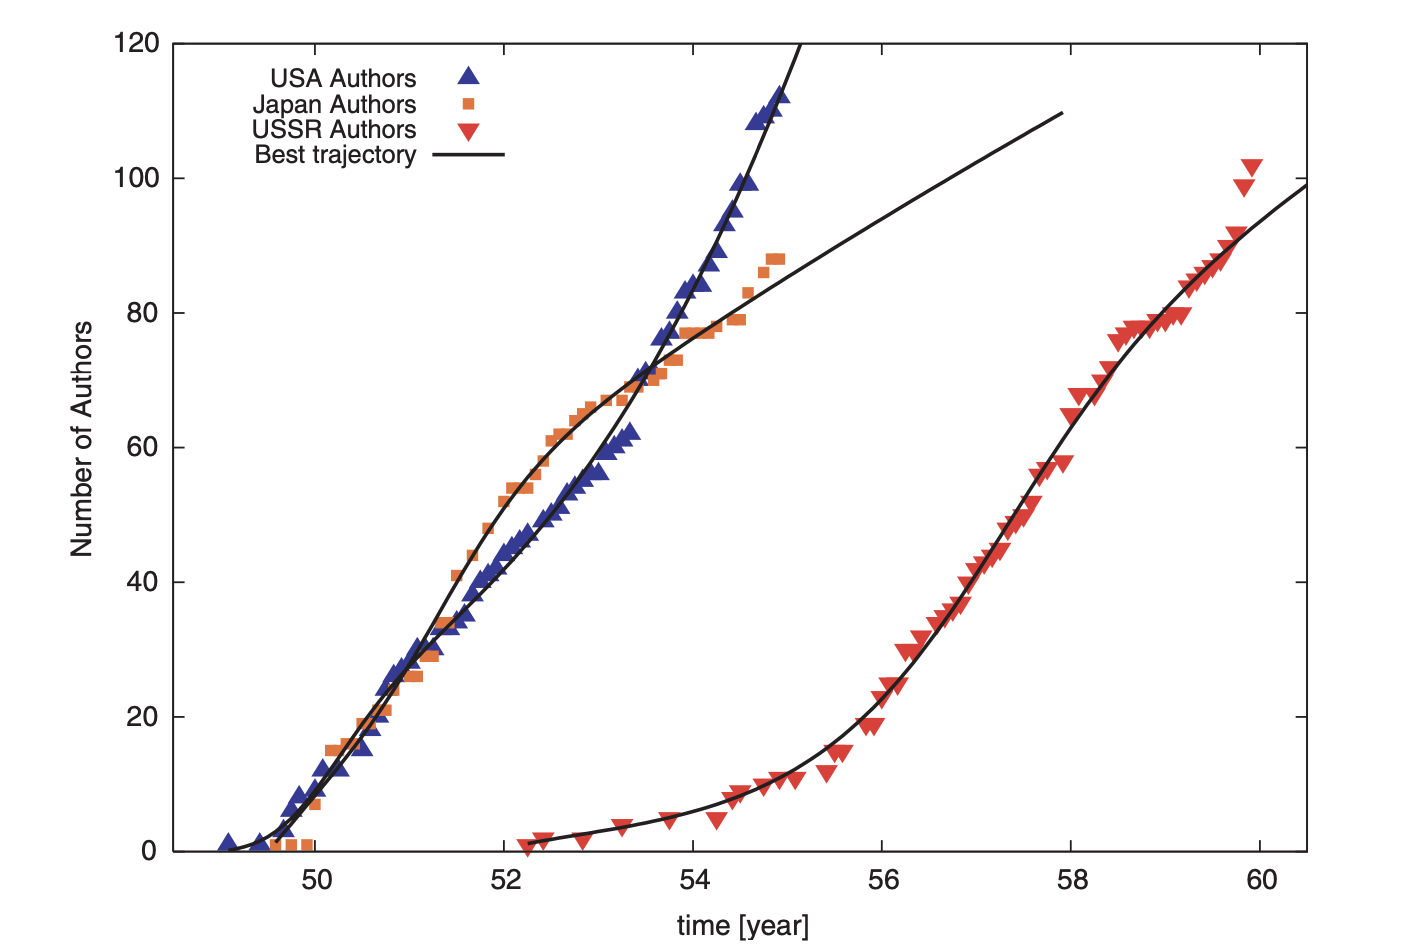
\includegraphics[width=\textwidth]{./figures/Feynman}}
    \begin{flushleft}{\footnotesize Note: \cite{bettencourt2006power}, showing their fitted SEIZ model to the diffusion dynamics of Feynman diagrams in theoretical physics communities}
    \end{flushleft}
  \end{figure}
\end{verbatimwrite}
\ifInBook{}{
}

Internet memes (\cite{dawkins1978selfish}) are a favorite topic of non-economist modelers. \IfPrivate{\href{https://github.com/iworld1991/EpiExp/blob/master/Literature/bauckhage2011insights.pdf}{\cite{bauckhage2011insights}}}{\cite{bauckhage2011insights}} shows that epidemiological models do a good job capturing the growth and decay of some famous memes. \cite{wang2011epidemiological} finds that a modified SIR model allowing for the reinfection of the ``recovered'' fits  the propagation dynamics of various viral memes well.   A large literature has followed their work. %\href{https://github.com/iworld1991/EpiExp/blob/master/Literature/kucharski2016modelling.pdf}{\cite{kucharski2016modelling}} fits an epidemiological model to outbreaks of notable internet contagions such as the ``ice bucket challenge'' and ``no-makeup selfies.''% suggesting an initial reproduction ratio in the range of 1.9 to 2.5.

%	\href{http://cs.stanford.edu/~ashton/pubs/twiral.pdf}{\cite{goel2016structural}} explores the structural factors (independent from the intrinsic properties of the content, nature of contact process, etc.) that seem to determine whether a news story spreads more effectively from a ``broadcast'' (common-source) or from a `viral' (person-to-person) mechanism.


% Internet memes are increasingly used to sway and manipulate public opinion. This prompts the need to study their propagation, evolution, and influence across the Web. In this paper, we detect and measure the propagation of memes across multiple Web communities, using a processing pipeline based on perceptual hashing and clustering techniques, and a dataset of 160M images from 2.6B posts gathered from Twitter, Reddit, 4chan's Politically Incorrect board (/pol/), and Gab, over the course of 13 months. We group the images posted on fringe Web communities (/pol/, Gab, and The_Donald subreddit) into clusters, annotate them using meme metadata obtained from Know Your Meme, and also map images from mainstream communities (Twitter and Reddit) to the clusters. Our analysis provides an assessment of the popularity and diversity of memes in the context of each community, showing, e.g., that racist memes are extremely common in fringe Web communities. We also find a substantial number of politics-related memes on both mainstream and fringe Web communities, supporting media reports that memes might be used to enhance or harm politicians. Finally, we use Hawkes processes to model the interplay between Web communities and quantify their reciprocal influence, finding that /pol/ substantially influences the meme ecosystem with the number of memes it produces, while \td has a higher success rate in pushing them to other communities.

% There is a methodological insight for economists in these studies: To the extent that certain classes or configurations of epidemiological models are found consistently to characterize the spread of non-economic ideas (even non-textual content like videos and images), economists might be well advised to select the models that generically perform well across many kinds of content.


% \begin{center}[Insert Figure \ref{fig:memes_curve} here]\end{center}

\begin{verbatimwrite}{./Slides/FigureMemesCurve}
\begin{figure}[!ht]
  \caption{ ~Virality of internet memes: \cite{bauckhage2011insights}}
  \label{fig:memes_curve}
    \subfloat[``salad fingers'']{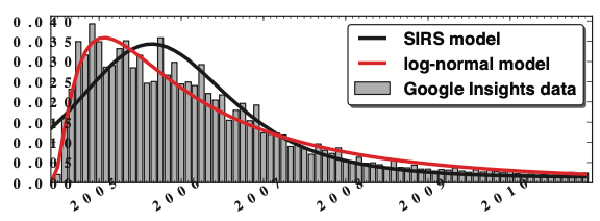
\includegraphics[width=\textwidth]{./figures/Memes1}}
    \newline
    \subfloat[``laughing baby'']{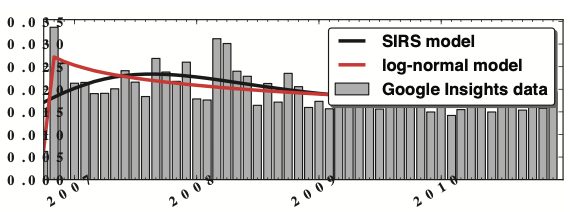
\includegraphics[width=\textwidth]{./figures/Memes2}}
    \newline
    \subfloat[``so much win'']{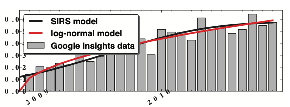
\includegraphics[width=\textwidth]{./figures/Memes3}}
    \begin{flushleft}{\footnotesize Note: This graph reproduces the SIRS model fit and log-normal fits to Google insights time series measuring the interest in six viral memes, as shown in  \cite{bauckhage2011insights}. }
    \end{flushleft}
\end{figure}

\end{verbatimwrite}
\ifInBook{}{
  {figure}[!ht] \centering \caption { ~Virality of internet memes: \href {https://github.com/iworld1991/EpiExp/blob/master/Literature/bauckhage2011insights.pdf}{\cite {bauckhage2011insights}}} \label {fig:memes_curve} \subfloat [``salad fingers'']{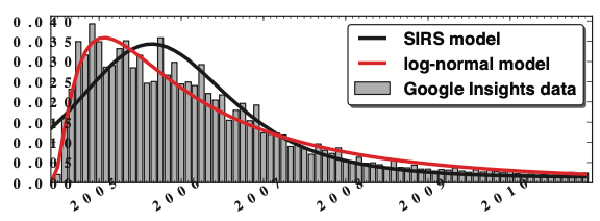
\includegraphics [width=\textwidth ]{./figures/Memes1}} \newline \subfloat [``laughing baby'']{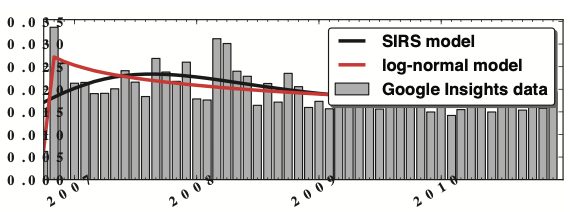
\includegraphics [width=\textwidth ]{./figures/Memes2}} \newline \subfloat [``so much win'']{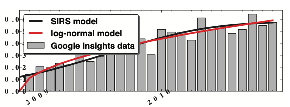
\includegraphics [width=\textwidth ]{./figures/Memes3}} \begin {flushleft}{\footnotesize Note: This graph reproduces the SIRS model fit and log-normal fits to Google insights time series measuring the interest in six viral memes, as shown in \cite {bauckhage2011insights}. } \end {flushleft} \end {figure} \end {verbatimwrite}{figure}[!ht] \centering \caption { ~Virality of internet memes: \href {https://github.com/iworld1991/EpiExp/blob/master/Literature/bauckhage2011insights.pdf}{\cite {bauckhage2011insights}}} \label {fig:memes_curve} \subfloat [``salad fingers'']{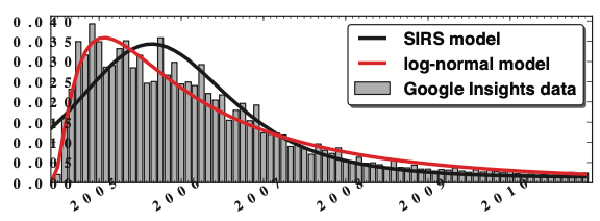
\includegraphics [width=\textwidth ]{./figures/Memes1}} \newline \subfloat [``laughing baby'']{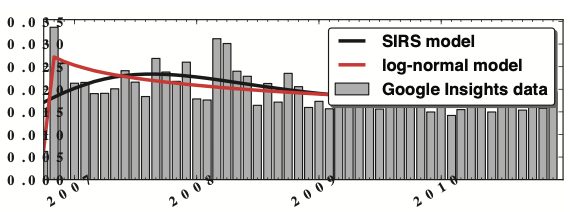
\includegraphics [width=\textwidth ]{./figures/Memes2}} \newline \subfloat [``so much win'']{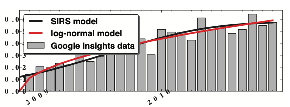
\includegraphics [width=\textwidth ]{./figures/Memes3}} \begin {flushleft}{\footnotesize Note: This graph reproduces the SIRS model fit and log-normal fits to Google insights time series measuring the interest in six viral memes, as shown in \cite {bauckhage2011insights}. } \end {flushleft} \end {figure} \end {verbatimwrite}{figure}[!ht] \centering \caption { ~Virality of internet memes: \href {https://github.com/iworld1991/EpiExp/blob/master/Literature/bauckhage2011insights.pdf}{\cite {bauckhage2011insights}}} \label {fig:memes_curve} \subfloat [``salad fingers'']{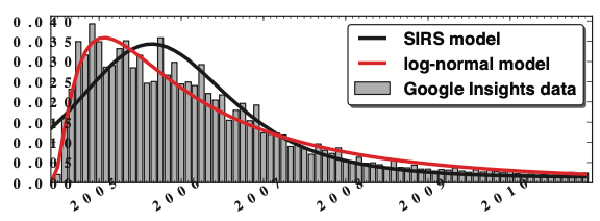
\includegraphics [width=\textwidth ]{./figures/Memes1}} \newline \subfloat [``laughing baby'']{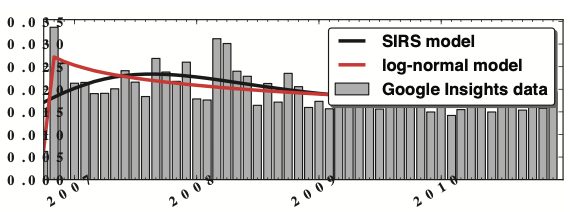
\includegraphics [width=\textwidth ]{./figures/Memes2}} \newline \subfloat [``so much win'']{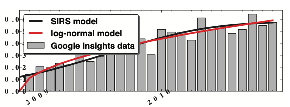
\includegraphics [width=\textwidth ]{./figures/Memes3}} \begin {flushleft}{\footnotesize Note: This graph reproduces the SIRS model fit and log-normal fits to Google insights time series measuring the interest in six viral memes, as shown in \cite {bauckhage2011insights}. } \end {flushleft} \end {figure} \end {verbatimwrite}\input {./Slides/FigureMemesCurve} 



 



 




  }
